\chapter{Verktøy}
\lhead{Verktøy}

\section{Utviklingsmiljø}
\subsection{Google App Engine SDK}
GAE (Google App Engine) kommer med et «Software Development Kit, SDK» og dette kan benyttes under utviklingen av applikasjoner som skal publiseres på GAE. SDK ’en gjør det mulig å lage et virtuelt miljø som fungerer på samme måte som miljøet som skal kjøre applikasjonen på nett. Her har man mulighet til å benytte seg av de aller fleste API som er knyttet til GAE. Denne kommer integrert med et grafisk grensesnitt man kan benytte, som gjør det mulig å se på logger produsert, oppdatere koden og se forandringer i sanntid, og direkte sende forandringer til den versjonen som ligger tilgjengelig i nettskyen.	  


 \begin{figure}[htbp]
	\centering
		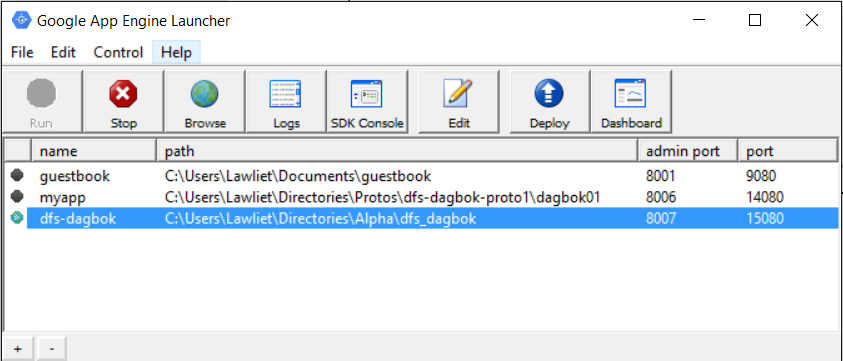
\includegraphics[scale=1.0]{gaesdk.png}
	\caption[Google App Engine SDK]{Grafisk grensesnitt for Google App Engine SDK.}
	\label{fig:gaesdk}
\end{figure}


\section{Editor}
\subsection{JetBrains PyCharm}
JetBrains PyCharm har blitt brukt som hoved-editor i utviklingsfasen. Denne editoren kommer rustet med mange funksjoner som hjelper til å skape en smidige utvikling, blant annet: bred kodefullføring, feil sjekking i sanntid, forslag til fikser av eventuelle problemer underveis, integrert git system for versjonskontroll, database tilkoblings muligheter, pakker til spesifikke web-rammeverker, med mer. 

\section{Version Control}
\subsection{Google App Engine Versioning.}
Google App Engine kommer med et system for å kunne adskille forskjellige versjoner av en applikasjon man laster opp. Her kan man velge mellom hvilken versjon som skal være offentlig, og man kan la en ny «Test» versjon kun være tilgjengelig for de brukere som får en link til denne versjonen. Dette systemet er på plass slik at man kan se hvordan en oppdatering oppfører seg i systemet, og man kan tillate noen utvalgte brukere muligheten til å teste og gi tilbakemeldinger på en nyere versjon av produktet før det taes i bruk offisielt.


\subsection{Git}
Git er et VCS (Version Control System), som har en hensikt av å lagre endringer i en fil eller et sett med filer over tid. Dette gjør det mulig å gå tilbake å se på tidligere versjoner av et prosjekt \citep{git:info}. Git ble først utviklet av Linus Torvalds i 2005, som hadde behov for et verktøy som kunne brukes til utviklingen av Linux \citep{git:history}. 


Git blir benyttet som en versjonskontroll over systemet, slik at man som utvikler kan lettere få en oversikt over systemets endringer over tid. Man har også muligheten til å utvikle i såkalte ‘branches’, som gjør det mulig å utvikle en ny feature ved siden av hovedprosjektet, og ikke plassere disse sammen før den nye feature er ferdig utviklet. Dermed blir det lettere å skille mellom utviklingsfasen og den fungerende hoved versjonen av et prosjekt.


\section{Oversikt med Jira}
Dette  prosjektet benytter systemet Jira til å holde oversikt over hvilke oppgaver det skal jobbes med, og antall timer logget  til prosjektet.

\subsection{Agile}
For å kunne ha orden i hvilke funksjonaliteter og oppgaver som skulle jobbes med blir Agile brukt. Agile er et system for å kunne legge inn oppgaver underveis i utviklingen som reflekterer hva som må jobbes med fremover i prosessen. Man kan splitte større funksjoner til mindre mer håndterlig oppgaver og på den måten få en bedre oversikt over progresjonen underveis i arbeidet.

\subsubsection*{Kanban}
Kanban er en underliggende metode innen Agile, og er basert på en dynamisk fremgangsmåte. Her har man mulighet til å fylle oppgaver inn i 4 felter som tilsier hvor i prosessen disse oppgavene er til enhver tid. Disse feltene består av: 

\begin{description}
\item[Backlog.]Oppgaver som skal  gjøres, men som ikke er prioritert for øyeblikket.

\item[Selected for Development.]Oppgaver som er utvalgt til arbeid så fort det er tid, dette er et slags mellomlagrings område som skiller ut det neste steget i utviklingen.

\item[In Progress.]Oppgaver som nå blir arbeidet mot, og man kan maks ha 5 oppgaver innen dette feltet til enhver tid.

\item[Done.] De ferdige oppgavene. Disse oppgavene ligger i dette feltet helt til en release forekommer. Det kan være logisk å jobbe med samme type oppgaver i én release, som bidrar til at når en release er sluppet, er det forekommet større arbeid innen minst én modul av prosjektet.
\end{description}


\subsection{Tempo}
Tidsskjema for prosjektet. Tempo vil kunne samarbeide med Agile, som gjør at når man legger inn timer direkte på en oppgave, vil dette registreres inn i Tempo og en timeliste blir generert.


\section{Design}
\subsection{Balsamiq Mockups 3}
Tidlig i utviklingsfasen ble det jobbet med et overordnet design nettsiden skulle ha, dette inkluderte en enkel oversikt over hvordan funksjoner kunne se ut, og visualisering av workflow brukerne skulle følge. Til dette ble Balsamiq Mockup 3 benyttet, som kunne benyttes i form av en 30 dagers prøve periode. Balsamiq Mockup er et program som er ment til å kunne la designet bli sketchet ut raskt og enkelt uten for mye detaljer. Det kan bli brukt som en metode å få idéer, og raskt teste ut hvordan dette kan se ut i virkeligheten.

\section{Grafer}
\subsection{Highcharts}
Highcharts er et grafisk data visualiseringsverktøy, utviklet av norske Highsoft. Utviklingen av Highcharts startet som et enkelt kartleggingsverktøy av snødybde målinger fra Vikjafjellet på hjemmesiden til eieren av Highsoft, Torstein Hønsi \citep{highcharts:info}. 


Highcharts er bygget i JavaScript og utarbeider interaktive grafer. Highcharts har en stor rekke forskjellige grafer som kan benyttes, bl.a.  linje, stolpe, pai diagram, og mange av disse kan kombineres i et. Dette er også åpen kildekode, som betyr at dersom man har lisens til å benytte produktet, har man muligheter til å gjøre egne forandringer direkte i koden \citep{highcharts:chart}. 

Da DFS selv har planer om å benytte Highcharts pakken på sine nettsider, ble vi enige om at det samme systemet skulle benyttes i treningsdagboken, da dette vil gjøre at brukerne vil kunne forholde seg til ett enkelt system for grafer.



\clearpage
\section{Django Pakker}
\subsection{Brukersystem}
\subsubsection*{Django-allauth}
Den mest brukte autentifiserings pakken tilgjengelig for Django utviklere \citep{allauth:package}. Den kommer integrert med bruker autentifisering, registrering, overordnet system for bruker kontroll for Admin og tredjeparts innloggings autentifisering \citep{allauth:git}. Dette prosjektet blir sponset av Nederlandske intenct \citep{allauth:sponsor} og er utviklet hovedsakelig av Nederlandske Raymon Penners, med samarbeid fra utallige andre i form bidrag på Github \citep{allauth:contrib}.

Denne pakken ble brukt som autentifiseringen i prosjektet. Django-allauth håndterer både de lokale brukerkontoer samt åpner for ekstern innlogging vha. Facebook.

%TODO: KILDER
%mestPop https://www.djangopackages.com/grids/g/authentication/
%[1] https://github.com/pennersr/django-allauth
%[2] http://www.intenct.info/
%[3] https://github.com/pennersr/django-allauth/graphs/contributors








